\documentclass{article}
\usepackage{cmap}
\usepackage{multicol}
\usepackage[top=3cm,bottom=3cm,left=2.95cm,right=2.95cm]{geometry}
\usepackage[hidelinks]{hyperref}
\usepackage{graphicx}
\usepackage{caption}
\usepackage{capt-of}
\newenvironment{Figure}
  {\par\medskip\noindent\minipage{\linewidth}}
  {\endminipage\par\medskip}

\title{Forrest Fire Simulation model}
\author{Tom Peerdeman - 10266185 \& Ren\'e Aparicio Saez - 10214054}

\begin{document}

\maketitle

\begin{abstract}
\textbf{\\In this paper the spread of forest fires is examined for a large variety of variables. Different types of grids are used, along with different types of vegetation, roads, water, probabilities of spreading and firefighters. By comparing different combinations of these variables, the impact of each variable can be examined and a general conclusion on how to slow down or even stop a forest fire could be made.}
\end{abstract}

\begin{multicols}{2}

\subsection*{Introduction}
Forest fires can spread in various ways and can be effected by a lot of environmental variables. Some variables are straight forward, as seen in the forest fire simulation made by Peerdeman\cite{oldcode}. Different neighborhoods and the density of a forrest are not just the only variables defining the spread of a forest fire. The way a fire spreads between flammable objects for example can make a huge difference in the way a forest fire moves. Fire can also be affected by environmental variables, like water, the weather or wind. Manmade objects and people can interfere with the fire as well. Firefighters can try to extinguish fire to keep the fire from spreading. Paths and roads, like water cannot be set on fire. It is however possible for fire to cross roads and some streams of water if the conditions are right. All these variables have to be taken into account when simulating a forest fire.\\\\
The experiments done in this paper are an expansion of the work done by Peerdeman\cite{oldcode}. The forest fire simulations are done by using cellular automata. Instead of using rules as was the case in the previous experiments, the experiments posed for this paper require probabilities. These probabilities are needed to simulate the environmental effects on the forest fire. By running various experiments and testing a variety of variables, it is possible to answer the question: "what variables have the biggest impact on the spread of a forest fire?".

\subsection*{Defining the neighborhoods}
\subsubsection*{Different grids}
In order to ensure that the simulation is applicable in many situations, three different types of grids were used to simulate forest fires. These grids are: the Cartesian grid, the hexagonal grid and the triangular grid. Each grid has a different spread of fire.\\\\
For the Cartesian grid a straightforward method is used. By using a Moore neighborhood the eight squares around the current square can be directly influenced. The neighborhood is shown in figure \ref{fig:cartesianstd}.\\\\
The hexagonal grid could be positioned in two different ways. Either with points facing up and down, or with points facing left and right. Both types of hexagons will do, by changing your perspective on the simulation, it is possible to simulate the other type of hexagon. For the experiments and simulations the type with points to the top and bottom is used. As shown by Hernandez et al. \cite{HernandezEncinas20071213}, hexagonal grids show a slight difference in mathematics when they are either odd or even (in this case along the x-axis). The neighborhood is shown in figure \ref{fig:hexstd}.  \\\\
Just like the hexagonal grid, the triangular grid can be placed in two different ways. Either with two of the points along the x-axis or two points along the y-axis. The first type is chosen, to keep consistency for all grids. Whereas the fire spread of the Cartesian and the hexagonal grids are the same, no matter the location, the spread of the triangular grid differs per position. The triangle can either point up or down, switching along each axis. The neighborhoods for the triangles are shown in figure \ref{fig:triangle1std} and figure \ref{fig:triangle2std}.
\begin{Figure}
 \centering
 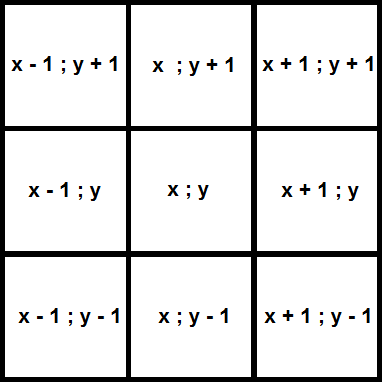
\includegraphics[width=0.79\textwidth]{imgs/cartesian.png}
 \captionof{figure}{Cartesian grid neighborhood}
\label{fig:cartesianstd}
\end{Figure}
\begin{Figure}
 \centering
 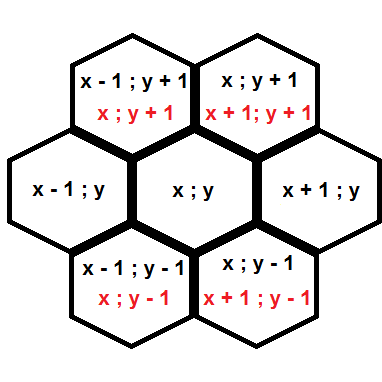
\includegraphics[width=0.79\textwidth]{imgs/hexagonal.png}
 \captionof{figure}{Hexagonal grid neighborhood}
\label{fig:hexstd}
\end{Figure}
\begin{Figure}
 \centering
 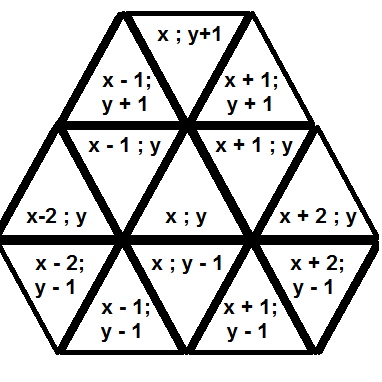
\includegraphics[width=0.79\textwidth]{imgs/triangle1.png}
 \captionof{figure}{Triangle 1 grid neighborhood}
\label{fig:triangle1std}
\end{Figure}
\begin{Figure}
 \centering
 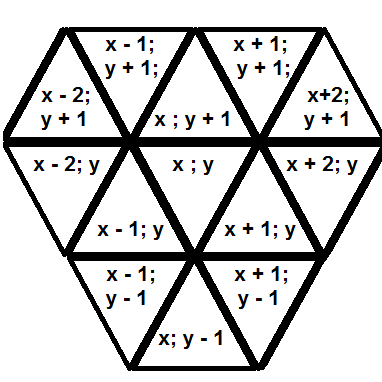
\includegraphics[width=0.79\textwidth]{imgs/triangle2.png}
 \captionof{figure}{Triangle 2 grid neighborhood}
\label{fig:triangle2std}
\end{Figure}

\subsubsection*{Spread probabilities}
Each grid can be initialized with certain probabilities for their neighborhoods. These probabilities represent the probability of fire to spread to the specific cell. By using probabilities, instead of a guaranteed fire spread, different types of situations can be used when simulating the fire. By changing the probabilities in certain ways, different types of weather, wind and terrain can be simulated. For example, when the weather is rainy, the probabilities can be set lower, while when it’s hot the probabilities can be set higher. The same goes for wind, if the wind blows in a certain direction, the probabilities for that direction can be set higher than the other directions.\\\\
In order to increase the environmental factor even more, it is also possible to influence cell's outside the neighborhood. In this way, extreme hot weather or high wind speeds can be simulated even better. When this feature is used, a new probability is created for fire to spread to a cell with a distance of two cell's from the current cell. This probability is calculated by dividing the interpolated probabilities of the cell's in the neighborhood in the direction of the cell outside the neighborhood by a given number. This way, the probability for fire to spread is always equal or lower to the probabilities of the cell's its probability was interpolated from.\\
The areas that could catch fire if the spread of distance two is enabled is shown in the following figures. Note that the area of the triangles is a bit odd. The area that would have been able to get on fire if all the surrounding cell's were used, was too big in comparison to the other grids. Because of that the area for the triangles has been reduced. The extended neighborhoods are shown in gray in figures \ref{fig:extcartesianstd},  \ref{fig:exthexstd},  \ref{fig:exttriangle1std} and  \ref{fig:exttriangle2std}.\\\\
Besides the increased environmental factor, the extended neighborhood also has as advantage that it can simulate fire moving across water and paths. This is a very useful feature. If this wasn't the case, fire could never spread even when facing a small river or path.\\\\
Firefighters also require a set of rules in order to move across the grid. Firefighters can only start their initial walk from the edge of a road. While they are moving along the road, they search their surrounding area for fire. If they notice a fire is in this area, they will start moving towards the fire. When the fire is reached, the fire fighter will try to extinguish the fire with a given probability. Besides the probability of the firefighter to extinguish the flames, it is also possible for the flames to kill the firefighter. The probability a firefighter will die is calculated by an exponential function. The more fire surrounds the fire fighter, the higher the probability he will die.
\begin{Figure}
 \centering
 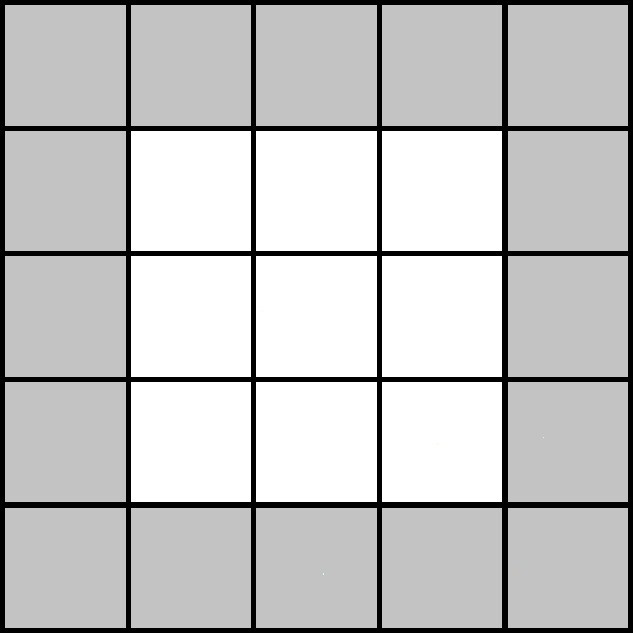
\includegraphics[width=0.79\textwidth]{imgs/extendedcartesian.png}
 \captionof{figure}{Extended Cartesian grid neighborhood}
\label{fig:extcartesianstd}
\end{Figure}
\begin{Figure}
 \centering
 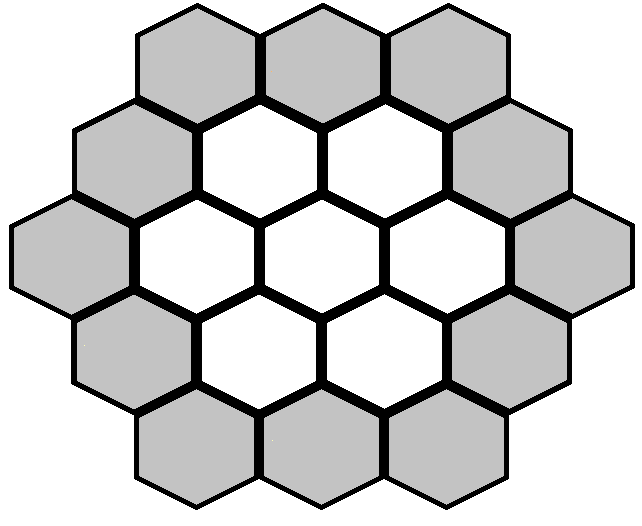
\includegraphics[width=0.79\textwidth]{imgs/extendedhexagonal.png}
 \captionof{figure}{Extended Hexagonal grid neighborhood}
\label{fig:exthexstd}
\end{Figure}
\begin{Figure}
 \centering
 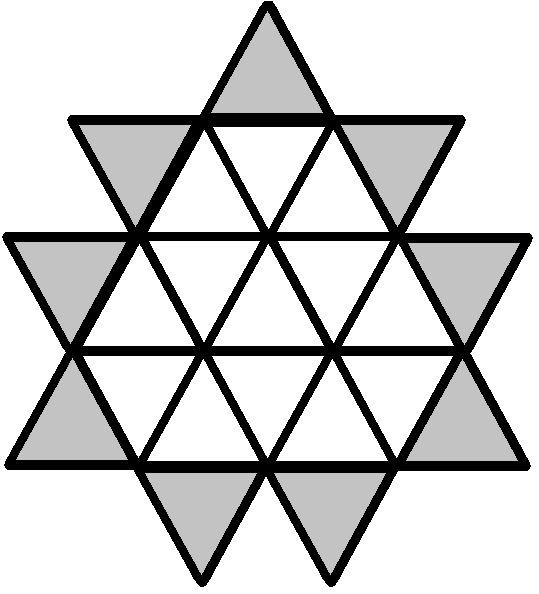
\includegraphics[width=0.79\textwidth]{imgs/extendedtriangle1.png}
 \captionof{figure}{Extended Triangle 1 grid neighborhood}
\label{fig:exttriangle1std}
\end{Figure}
\begin{Figure}
 \centering
 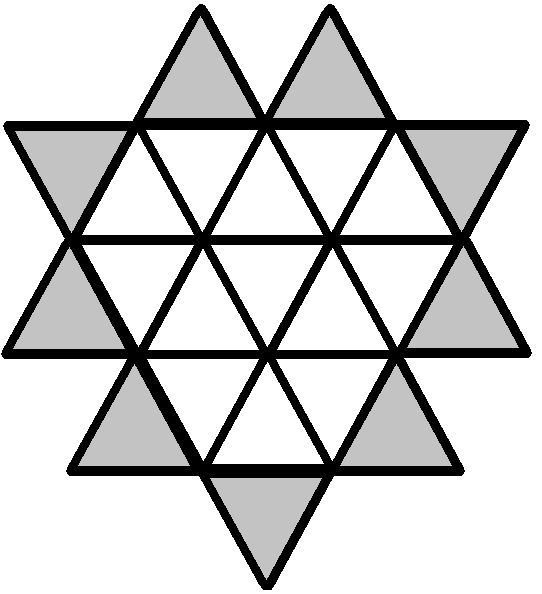
\includegraphics[width=0.79\textwidth]{imgs/extendedtriangle2.png}
 \captionof{figure}{Extended Triangle 2 grid neighborhood}
\label{fig:exttriangle2std}
\end{Figure}

\subsection*{Experiments}
Some basic experiments are already done for the Cartesian grid in the work of Peerdeman \cite{oldcode}. In addition to the experiments already made for the Cartesian grid, the same experiments have to be done for the other grids. Besides reproducing the same experiments for the other grids, new experiments can be done. The new variables create a huge variety in possible experiments. To expand the made experiments, the most logical addition is to gradually add variables and to look at the impact of these variables on the known results.\\\\

\subsubsection*{Basic experiments}
To start off, results are needed for a simulation on a simple forest, without any roads or streams of water running through the forest. Even though the results for the Cartesian grid are already known the experiments are made for all the grids, to ensure consistency in the experiments. Each simulation is run 50 times. This is done to overcome coincidental spreads and to show a more generalized view for each result.\\\\
By increasing the density gradually after each run of simulations a variety of information van be analyzed. It is possible to look at the percentage of the forest that is burned, the percentage of simulations where the fire reached the other side of the grid and the time in ticks it took to reach the other side of the grid.

\subsubsection*{Additional Experiments}
After the basic experiments are done, variables can be added to the simulations. The first variable to be added is the enlarged distance for fire to spread to more neighbors. This variable will increase the speed of the fire. Again the density is increased after every set of simulation runs.\\\\
The second variables to be added are roads and streams of water. These variables are tested with and without the additional distance for fire to spread. Without the additional distance, the addition of roads and water will most likely bring on problems for the simulation. Fire cannot spread across water or roads if it isn't allowed to move an extra square to each side. This will change when the additional distance is enabled again.\\\\
After these experiments are done, there is a final variable, the firefighters, that could change the spread of fire. Again two experiments have to be made, one with and one without the additional distance. With these final experiments a conclusion can be made about the impact of each variable on the spread of fire.

\subsubsection*{Expected results}
It is expected that the fire will spread the fastest for the grid with the most neighbors. The amount of neighbors depends on the additional distance that is used for some experiments. As shown, the Cartesian grid has 8 neighbors directly surrounding the cell. If the distance is increased, the number of neighbors increases to 24 neighbors that can catch fire. For the hexagonal grid this is 6 neighbors directly surrounding the cell and a total of 18 when the distance is increased. Finally the neighborhood of the triangular grid starts with 12 neighbors directly surrounding the cell and 21 neighbors with an increased distance.\\\\
As can be seen from the amount of neighbors it is expected that, without the additional distance, the triangular grid will have the fastest spread of fire, followed by the Cartesian grid and the hexagonal grid. When the distance is increased, the amount of neighbors for the Cartesian grid increases to a point where it's amount of neighbors is greater than the amount of neighbors for the other grids. Because of this is can be expected that the Cartesian grid will move faster with the increased distance enabled, followed by the triangular grid and the hexagonal grid being the slowest.\\\\
It is also expected that the percentage of forest that will burn down will depend on the amount of neighbors surrounding a cell. Therefore a coherence is expected in the percentage of the forest that is burned and the speed the forest fire will spread.\\\\
Besides the additional distance variable, the addition of roads and streams of water will affect the speed of the fire spread as well. By adding roads and streams of water, the fire will be slowed down. Depending on the distance the fire can travel from a cell, the fire will either be stopped by the roads and water or slowed down by the fact that the probability to cross the water or the road is lower than moving to a cell closer to the current cell. It can therefore be expected that the addition of water will drastically interfere with the speed and the percentage of the forest that is burnt when the fire can only spread to the direct neighbors. It is expected that with the water and paths enabled and also the distance increased, the fire will move a bit slower than without the water and paths. However the percentage that will get burned down will remain around the same as without water or roads.
The final variable, the firefighters, will interfere with the spread of fire and the percentage that will get burned. When only the surrounding cells can be set on fire, the firefighters will most likely lower the percentage of the forest that will get burned. The fire will spread less fast when facing firefighters as well. However, because firefighters will walk along the roads, the fire will only be stopped around the roads. Therefore the firefighters will not provide a very big impact, compared to the same experiment without the firefighters.\\\\
When the firefighters are added and the additional distance is used, the fire will again be slowed down and a lower percentage of the forest will get burned. However, the fire will most likely still burn down a large amount of forest, due to the bigger area a fire can spread to compared to the slow speed a fire fighter can move towards a fire. It is therefore expected that a firefighter only has a small impact on the speed of the fire and percentage of forest that will get burned.


\subsection*{Results\footnote{Only the most interesting and useful results are. All results are listed at the git repository \url{https://github.com/TomPeerdeman/ProjectCompScience/tree/master/Report/imgs/plot}}}
\subsubsection*{Experiment 1}
As expected, the triangular grid has a more rapid spread of fire compared to the other grids for the first experiment. Every grid type shows a similar kind of graph. A small fraction of forest burned with low densities, followed by a rapid increase in the burned fraction at some density. This increase differs per grid type. The triangular grid type has a rapid increase around a density of 0.45 to 0.5 percent forest density. Whereas the Cartesian grid has an increase around 0.6 to 0.65 and the hexagonal grid at 0.75 to 0.8 percent forest density. This is shown in figure \ref{fig:ex1frac}. It is also notable that at the same time the fraction of forest that is burned rapidly increases, the opposite side of the forest is reached.

\begin{Figure}
 \centering
 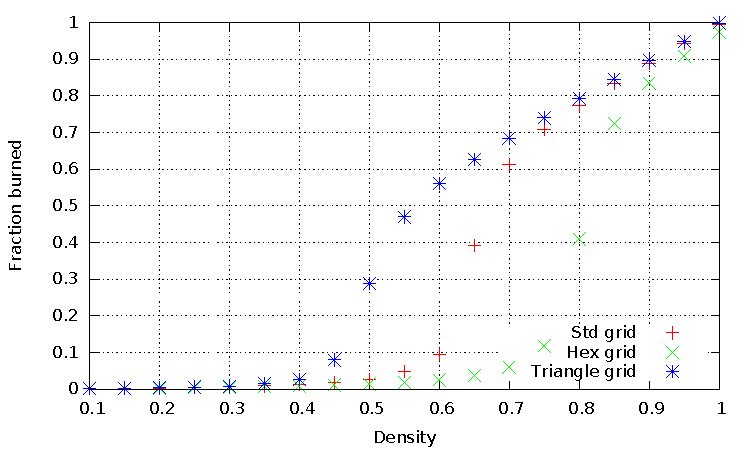
\includegraphics[width=\textwidth]{imgs/plot/ex1/fracburned.pdf}
 \captionof{figure}{Average fraction of the trees burned for experiment 1}
\label{fig:ex1frac}
\end{Figure}
\subsubsection*{Experiment 2}
While the first experiment only had a small neighborhood for the spread of fire, the second experiment has an increased neighborhood. The rapidly increasing fraction of burned forest has now moved to a lower forest density. This is shown in figure \ref{fig:ex2frac}. The standard grid now starts the increase before the triangular grid, followed by the hexagonal grid, as was expected. It is however notable that after a small rapid increase in the fraction of forest that is burned, the increase in fraction burned becomes linear. This linear increase seems to be equal for all grid types. It is also notable that after the rapid increase occurred, the opposite side of the forest is being reached in almost all cases.

\begin{Figure}
 \centering
 \includegraphics[width=\textwidth]{imgs/plot/ex2/fracburned.pdf}
 \captionof{figure}{Average fraction of the trees burned for experiment 2}
\label{fig:ex2frac}
\end{Figure}
\subsubsection*{Experiment 3}
By adding water and roads to the grids, and reducing the distance the fire can spread to the current cells, the increase in the burned fraction of forest changes a lot compared to the first experiment. The rapid increase in the fraction burned seems to be either completely gone or really weak as shown in figure \ref{fig:ex3frac}. The increase looks more linear than exponential when it starts increasing. The increase also starts at a higher density than before, as was expected. Where the results from experiment 1 and experiment 2 showed clean graphs, the results for experiment 3 show more anomalies at higher densities. This can be explained when looking at figure \ref{fig:ex3opp}, the results of the graph showing the percentage of forest fires that reached the opposite side of the forest. It becomes clear that the opposite side is never reached in all cases, no matter what the density of the forest may be. This has to do with the fact that the forest fires cannot cross water or roads. When higher densities of vegetation occur, parts of the grid cannot be accessed because of water or roads.
\begin{Figure}
 \centering
 \includegraphics[width=\textwidth]{imgs/plot/ex3/fracburned.pdf}
 \captionof{figure}{Average fraction of the trees burned for experiment 3}
\label{fig:ex3frac}
\end{Figure}

\begin{Figure}
 \centering
 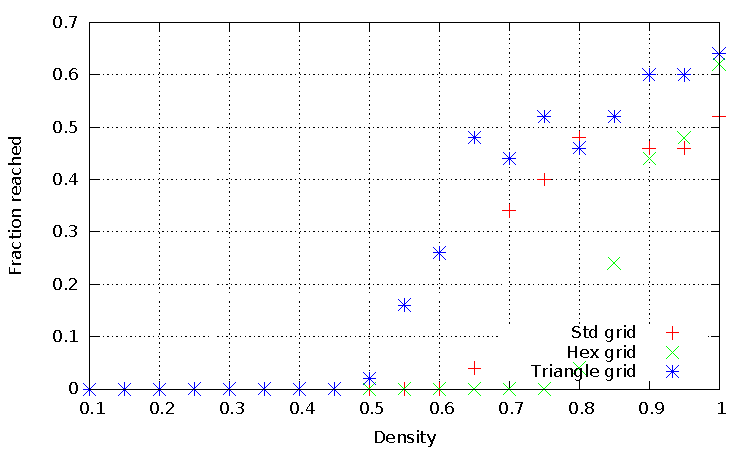
\includegraphics[width=\textwidth]{imgs/plot/ex3/oppreached.pdf}
 \captionof{figure}{Percentage of simulations where the fire reached the opposite of the grid for experiment 3}
\label{fig:ex3opp}
\end{Figure}
\subsubsection*{Experiment 4}
Because it was already expected that experiment 3 would cause problems in moving past water, experiment 4 was done with an increased distance for the spread of fire. When comparing the results shown in figure \ref{fig:ex4frac} with the results of experiment 2, it becomes clear that when water and roads are added, fire does move slower over the grid. The increase still starts off with a small exponential growth, shortly after followed by a linear increase. But the increase starts at a higher density compared to experiment 2. The same goes for the fraction of runs that reached the opposite side of the forest. Compared to the second experiment, the density has to be a bit higher in order for a fire to reach the opposite side when it has to cross water and roads.

\begin{Figure}
 \centering
 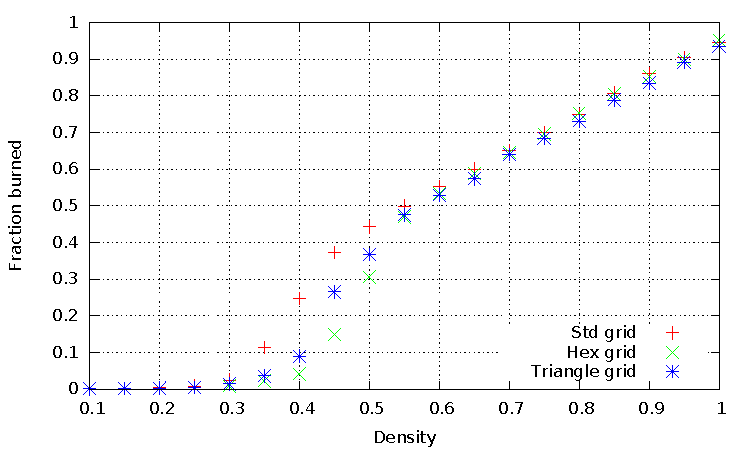
\includegraphics[width=\textwidth]{imgs/plot/ex4/fracburned.pdf}
 \captionof{figure}{Average fraction of the trees burned for experiment 4}
\label{fig:ex4frac}
\end{Figure}
\subsubsection*{Experiment 5}
By adding firefighters to the grids, and the distance for the spread of fire again lowered to the surrounding cells, a comparison can be made with experiment 3. The increase in the fraction of forest that is burned starts at the same moment as with experiment 3 as shown in figure \ref{fig:ex5frac}. This can be explained by the fact that firefighters only spawn at the edge of the grid. Because of that the extinguishing will most likely start when the fire has already been spreading for a while. It can also be explained by the randomizing of the grids. Since the fire cannot spread across water or roads, certain parts of the map will become inaccessible for the fire. It is possible that for this experiment more maps had inaccessible locations compared to experiment 3. Overall a lower fraction is burned at higher densities than before. This was expected since firefighters will extinguish more fire when there is more fire. This can also be observed by the difference in the results of experiment 3 and experiment 4. While experiment 4 shows a clean increasing linear line for the fraction that was burnt, the increase for experiment 3 doesn't increase in a linear fashion at all.

\begin{Figure}
 \centering
 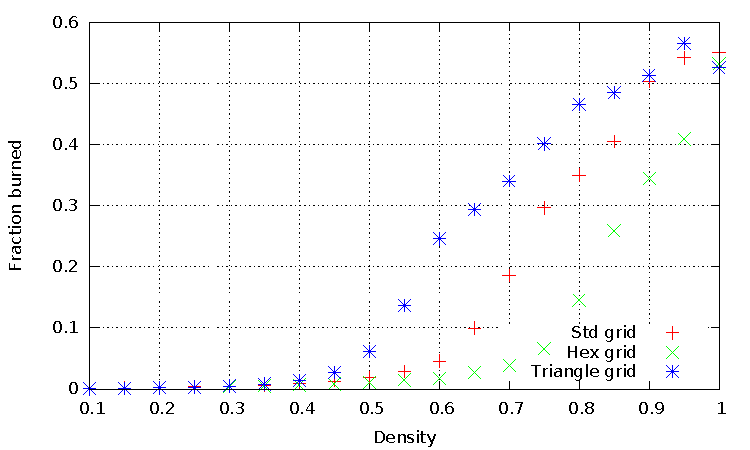
\includegraphics[width=\textwidth]{imgs/plot/ex5/fracburned.pdf}
 \captionof{figure}{Average fraction of the trees burned for experiment 5}
\label{fig:ex5frac}
\end{Figure}
\subsubsection*{Experiment 6}
When the distance fire can spread is increased to the larger neighborhood, the effect of firefighters decreases as shown in figure \ref{fig:ex6frac}. The overall fraction burned for each density is a bit lower when compared to the results of experiment 4. However the difference is almost too small to notice when comparing the graphs. The impact of firefighters is therefore, as was expected, low and could even be disregarded. The low impact of firefighters can be explained by the fact that the fire can spread over a distance of two squares, while the firefighter can only move one square. The fire will therefore move faster than the firefighter, lowering the impact of the firefighter.

\begin{Figure}
 \centering
 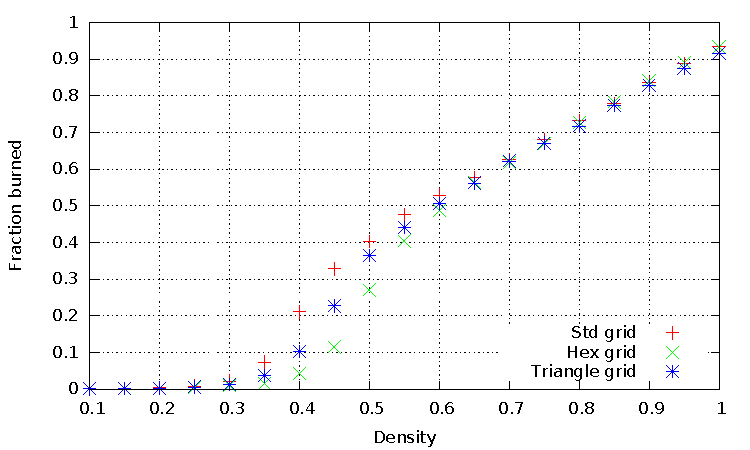
\includegraphics[width=\textwidth]{imgs/plot/ex6/fracburned.pdf}
 \captionof{figure}{Average fraction of the trees burned for experiment 6}
\label{fig:ex6frac}
\end{Figure}
\subsection*{Discussion}
The main problem in the simulation lies with the impact of firefighters on the spread of fire. The difference in results is around 5\%, which is so small that it could be mathematically disregarded. However, if the firefighters were simulated in another way, their impact might increase. The current simulation only spawns firefighters at the edges of the grid. Firefighters can move one square for every time step. The same goes for fire (if the probability to spread is reached). When the extended spread distance is enabled, it is even possible for fire to spread more than one square. Firefighters therefore have a disadvantage compared to the fire. Another problem for the firefighters is the fact that when he notice\\\\ 
Besides the disadvantage in speed for the current firefighters, other methods of firefighting could change the spread of fire. It is common to use airplanes or helicopters to extinguish large forest fires. This method of firefighting however is not available in the current simulation. By changing the speed of the firefighters and combining forces with other firefighters, the impact will most likely be higher than the current impact on the speed of the spread of fire.\\\\
Apart from the firefighters, other experiments could be done to find out how different combinations of variables impact the spread of fire. The probabilities implemented in the simulations were not used in the current experiments, but could be used in other experiments to simulate weather effects like rain or wind.\\\\
For the current simulation program was build on top of the old code. Because of this method of implementing new code, certain aspects were more difficult to implement. By not changing the old code and just extending it, an extra unnecessary difficulty was created. If a new simulation process for firefighters is created it is therefore advised to simply adjust the current code instead of extending it.

\subsection*{Conclusion}
From the experiments we can conclude that the biggest impact on the spread of fire is the presence of roads and water. When roads and water are added to the forest fire simulation, the spread of fire either completely stops the spread to parts of the forest or is slowed down significantly when moving across the road or streams of water. It also becomes clear that the firefighters have such a small impact that their interference can even be disregarded. A change of about 5\% is significantly too small to make a difference in the results. Therefore further research could be made with other firefighting algorithms.\\\\

\nocite{*}
\bibliographystyle{plain}
\bibliography{Forest_fire_paper}
\end{multicols}

\end{document}
